% Section 4.4: Weight Optimization
\subsection{Weight Optimization}
\label{sec:weight_optimization}

The edge scoring function (Section~\ref{sec:edge_scoring}) combines the features selected by the feature audit (Section~\ref{sec:feature_selection}) into a weighted sum. Rather than hand-tune these weights, we optimize them with Nelder-Mead simplex search~\cite{neldermead1965}, a derivative-free method suited to the noisy, non-convex AUC surface over a weighted combination of heterogeneous features.

\textbf{Objective.}
Given a feature matrix $\mathbf{F} \in \mathbb{R}^{m \times k}$ (valid edges only, after filtering self-loops and user edges) and binary labels $\mathbf{y} \in \{0,1\}^m$ from red-team ground truth, we find weights $\mathbf{w}^* = (w_1, \dots, w_k)$ that maximize ROC AUC:
\begin{equation}
\mathbf{w}^* = \arg\max_{\mathbf{w}} \; \text{AUC}\!\left(\mathbf{y},\; \sum_{i=1}^{k} w_i \cdot f_i(\mathbf{F})\right)
\end{equation}
where $f_i$ is the $i$-th feature column. Non-binary features receive a percentile rank transform before scoring to reduce outlier influence; binary features pass through unchanged.

\textbf{Procedure.}
The optimizer starts with equal weights $w_i = 1/k$ and runs Nelder-Mead with adaptive step sizes for up to 500 iterations (convergence tolerances: $\text{xatol} = 10^{-6}$, $\text{fatol} = 10^{-8}$). Each iteration computes a weighted score vector and evaluates AUC. The best weights seen during the search are retained, even if the final simplex iteration doesn't improve.

\textbf{Integration.}
Optimization runs once per pipeline execution, after feature extraction and before edge scoring. The optimized weights go directly to the scoring function. If optimization fails (e.g., insufficient label diversity), the pipeline falls back to equal weights with a logged warning.

\textbf{Output artifacts.}
The optimizer logs per-iteration weights, AUC, and convergence status. Final results include the optimized weight vector, per-feature weighted contributions, and a comparison of AUC improvement from equal to optimized weights.

\begin{figure}[htbp]
\centering
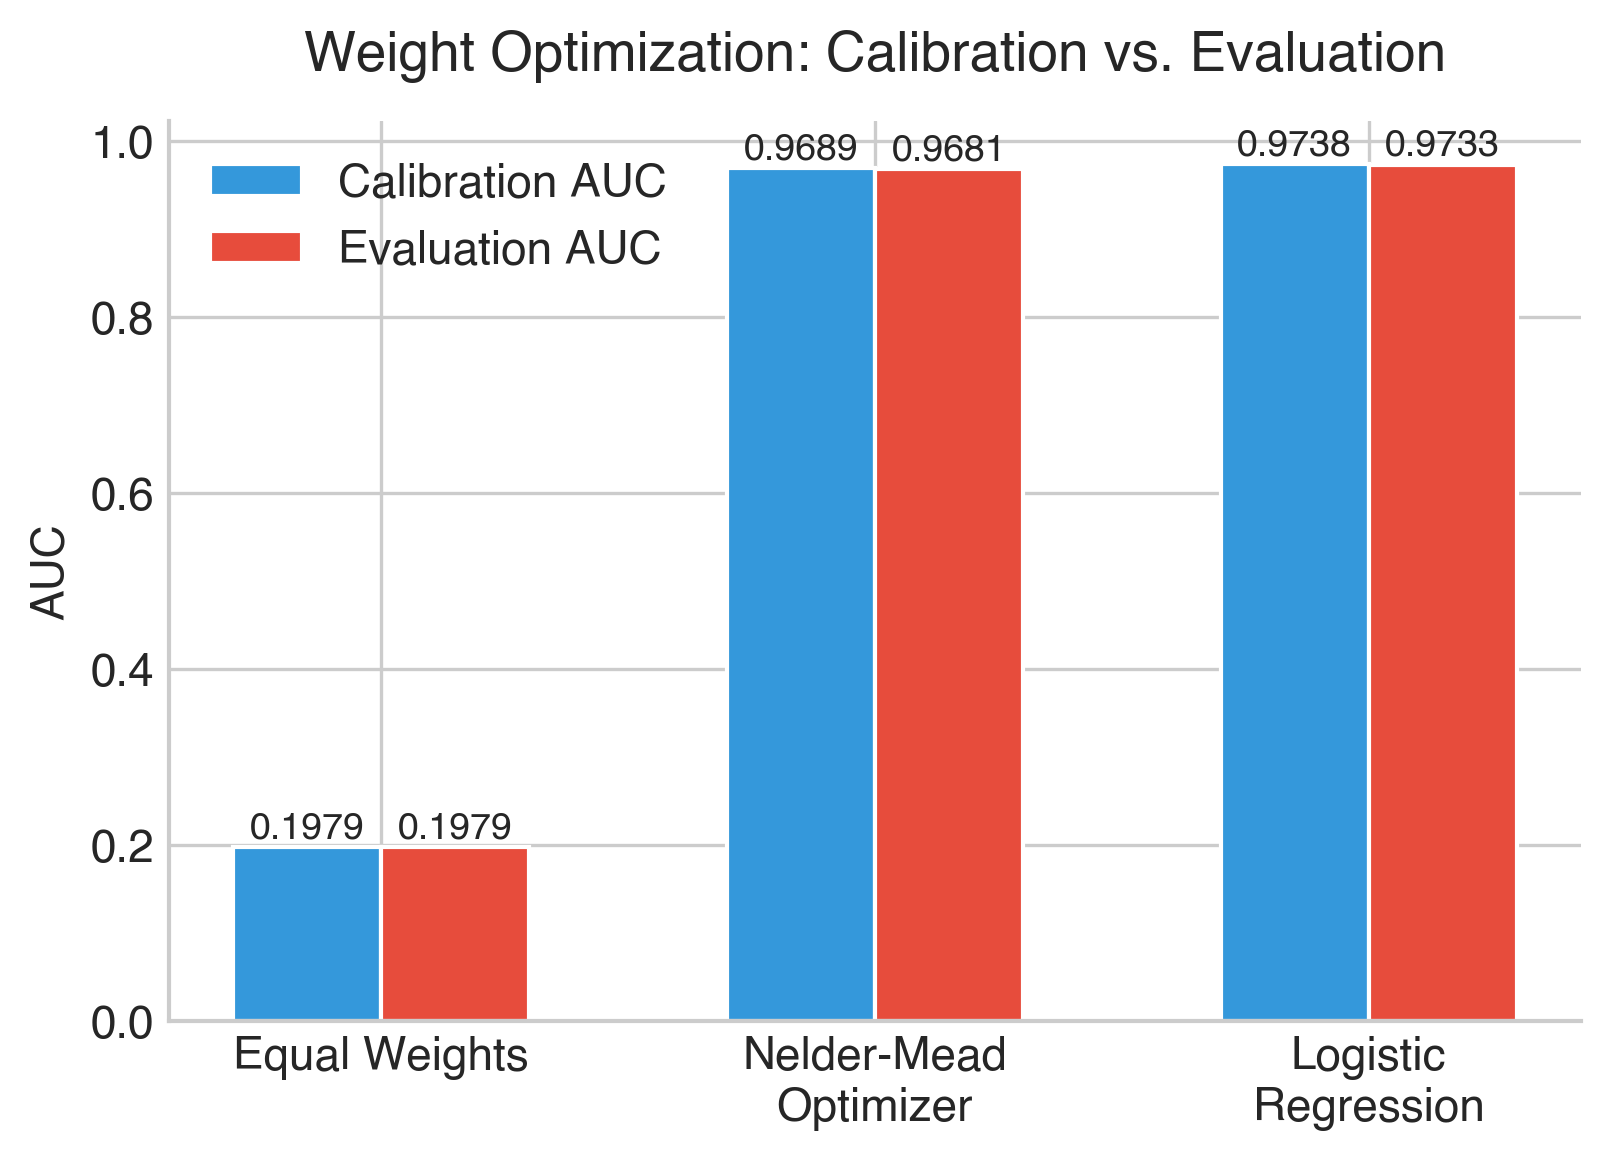
\includegraphics[width=0.95\columnwidth]{figures/weight_optimization.png}
\caption{Nelder-Mead optimization trajectory. Per-iteration ROC AUC over the weight space, starting from equal initialization.}
\label{fig:weight_optimization}
\end{figure}

\textbf{Feature audit connection.}
The optimized features are those the held-out AUC audit selected (Section~\ref{sec:feature_selection}). These span authentication semantics, graph structure, and host behavior, the three signal categories the audit found most discriminative.
